\section{Pysical Objects}

Using some similar technology to the iDummy\footnote{"IDummy" IDummy Product Website, 2015, accessed November 05., 2016, \url{http://www.idummy.com/}} one can create various objects of different size and shape. A user wearing a VR Headset can see a specific object and feel it as if it was the real thing. Using the technology developers can extend the realm of VR to one more dimension.

Using something similar to the modular tiles creating levels in portal (a 100x100 cm tile is attached to a robotic arm)

\begin{figure}
	\centering
	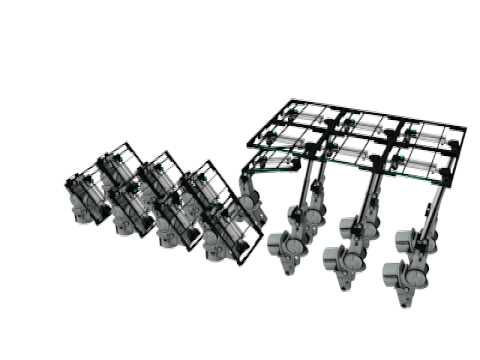
\includegraphics[width=0.9\columnwidth]{./figures/hqdefault}
	\caption{Foobar}~\label{fig:figure2}
\end{figure}

I can think of an application where the tiles are intelligently configured to 'disapear' (into the ground) behind the player and appear in front of him (out of the ground again) kind of like a hamster wheel, macking the playable area seem infinitely large to the player.

Minor field: hearing combined with VR games
